% Figure 1: the comparison (schematic, no data). Compiled inline with TikZ.
\usetikzlibrary{arrows.meta,positioning,calc,fit}
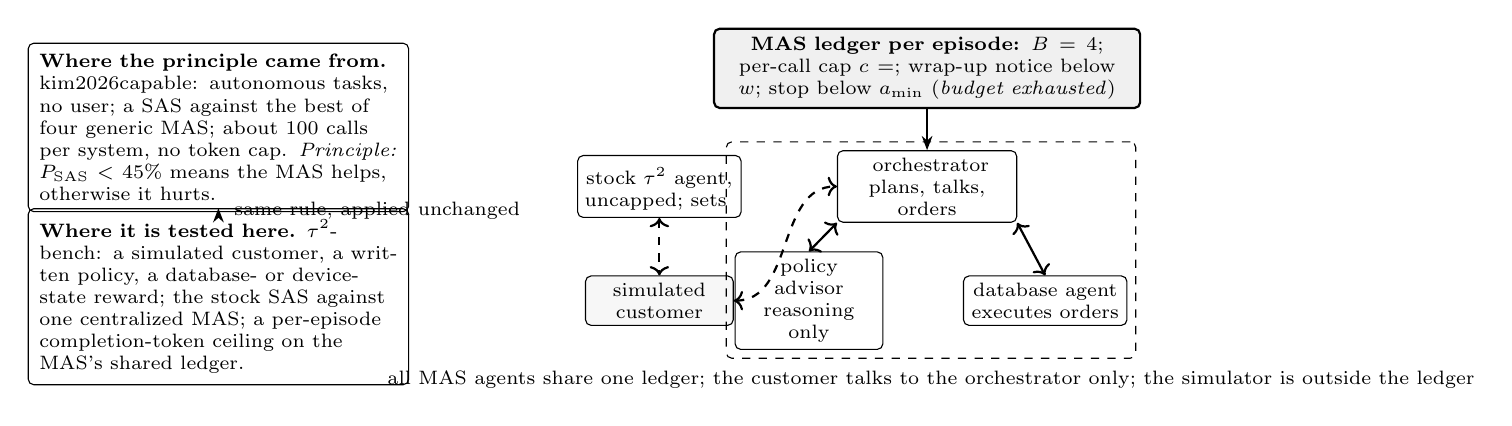
\begin{tikzpicture}[
  font=\scriptsize,
  box/.style={draw, rounded corners=2pt, align=left, inner sep=4pt, text width=4.55cm},
  comp/.style={draw, rounded corners=2pt, align=center, inner sep=2.5pt, minimum height=0.55cm, fill=white},
  ledger/.style={draw, thick, rounded corners=2pt, align=center, inner sep=3pt, fill=black!6},
  arr/.style={-{Stealth[length=1.8mm]}, thick}
]
% ---- left panel
\node[box] (kim) at (0,0.15) {\textbf{Where the principle came from.} \citet{kim2026capable}: autonomous tasks, no user; a SAS against the best of four generic MAS; about 100 calls per system, no token cap. \emph{Principle:} $P_{\mathrm{SAS}} < 45\%$ means the MAS helps, otherwise it hurts.};
\node[box] (here) at (0,-2.0) {\textbf{Where it is tested here.} $\tau^2$-bench: a simulated customer, a written policy, a database- or device-state reward; the stock SAS against one centralized MAS; a per-episode completion-token ceiling on the MAS's shared ledger.};
\draw[arr] (kim.south) -- node[right, xshift=2pt] {same rule, applied unchanged} (here.north);

% ---- right panel
\node[ledger, text width=5.2cm] (ledg) at (9.0,0.9) {\textbf{MAS ledger per episode:} $B = 4\Bx$; per-call cap $c=\Bx$; wrap-up notice below $w$; stop below $a_{\min}$ (\emph{budget exhausted})};
\node[comp, text width=1.9cm] (s1) at (5.6,-0.6) {\textbf{\Sone} \\ stock $\tau^2$ agent, uncapped; sets $\Bx$};
\node[comp, text width=2.1cm] (orch) at (9.0,-0.6) {\textbf{\Mone} orchestrator \\ plans, talks, orders};
\node[comp, text width=1.7cm] (adv) at (7.5,-2.05) {policy advisor \\ reasoning only};
\node[comp, text width=1.9cm] (db) at (10.5,-2.05) {database agent \\ executes orders};
\node[comp, fill=black!3, text width=1.7cm] (usr) at (5.6,-2.05) {simulated customer};
\draw[arr] (ledg.south -| orch) -- (orch.north);
\draw[arr, <->] (orch.south west) -- (adv.north);
\draw[arr, <->] (orch.south east) -- (db.north);
\draw[arr, <->, dashed] (s1.south) -- (usr.north);
\draw[arr, <->, dashed] (usr.east) to[out=0,in=180] (orch.west);
\node[draw, dashed, rounded corners=2pt, fit=(orch)(db)(adv), inner sep=3pt] (MAS) {};
\node[below=1pt of MAS, font=\scriptsize] {all MAS agents share one ledger; the customer talks to the orchestrator only; the simulator is outside the ledger};
\end{tikzpicture}
